%%%%%%%%%%%%%%%%%%%%%%%%%%%%%%%%%%%%%%%%%%%%%%%%%%%%%%%%%%%%%%%%%%%%%%%%
%Desarrollo de un juego para Nintendo DS | Trabajo de Fin de Grado
% Escuela Politécnica Superior de la Universidad de Alicante
% Realizado por: Carla Maciá Díez
% Contacto: carlamd1997@hotmail.com / cmd23@alu.ua.es
%%%%%%%%%%%%%%%%%%%%%%%%%%%%%%%%%%%%%%%%%%%%%%%%%%%%%%%%%%%%%%%%%%%%%%%%

\chapter{Diseño del juego (Game Design Document)} 

\subsection{Características}

\begin{itemize}
    \item \textbf{Título:} Touch \& Brush.
    \item \textbf{Plataforma:} Familia de consolas Nintendo DS.
    \item \textbf{Genero:} Agilidad mental.
    \item \textbf{Audiencia:} Todas las edades.
    \item \textbf{Idioma:} Inglés.
\end{itemize}

\vspace{1cm}


\subsection{Historia}

Un día cualquiera en un \textbf{museo de arte tradicional} sucedió una catástrofe. Un malvado pincel robó toda la pintura de los \textbf{cuadros} de la exposición haciendo que estos se volviesen \textbf{furiosos}, se separasen de las paredes que los sostenían y empezaran a atacar a la gente.

\vspace{0.5cm}


\textbf{Cherry}, una pequeña niña que disfrutaba de una agradable excursión al museo ese día con su clase, al ver la situación de pánico decide actuar. Es entonces cuando se encuentra con otro pincel, llamado \textbf{Celio}, que le asegura a la chica que la única manera de devolver los cuadros a la normalidad es pintarles lo que ellos quieran. Así pues, Cherry y Celio deciden trabajar juntos para salvar el museo.

\vspace{1cm}


\subsection{Ambientación y estilo}

Al tratarse de un juego 2D para la consola Nintendo DS, el estilo que adoptarán los escenarios y personajes de Touch \& Brush será \textbf{pixelart\footnote{Estilo de arte digital que trabaja con las imágenes a nivel de pixel.} y  cartoon\footnote{Estilo de dibujo y estilización de personajes de personajes con proporciones irreales de tal manera que llega incluso a tener un carácter humorístico y simpático.}}, ya que el tamaño de nuestra pantalla y sprites es reducido.

\vspace{0.5cm}

El juego se desarrolla en el espacio cerrado de un museo de arte, así que el fondo principal donde se desarrolla el gameplay se trata de una de sus salas. Esta misma poseerá las características más típicas de un museo de arte, como puede ser un reluciente parqué, una ténue iluminación con puntos de luz hacia la pared donde deberían ir los cuadros y un fondo azul oscuro para que los sprites y elementos por encima de éste resalten sin problema.

\vspace{0.5cm}

\begin{figure}[htbp]
\centering
  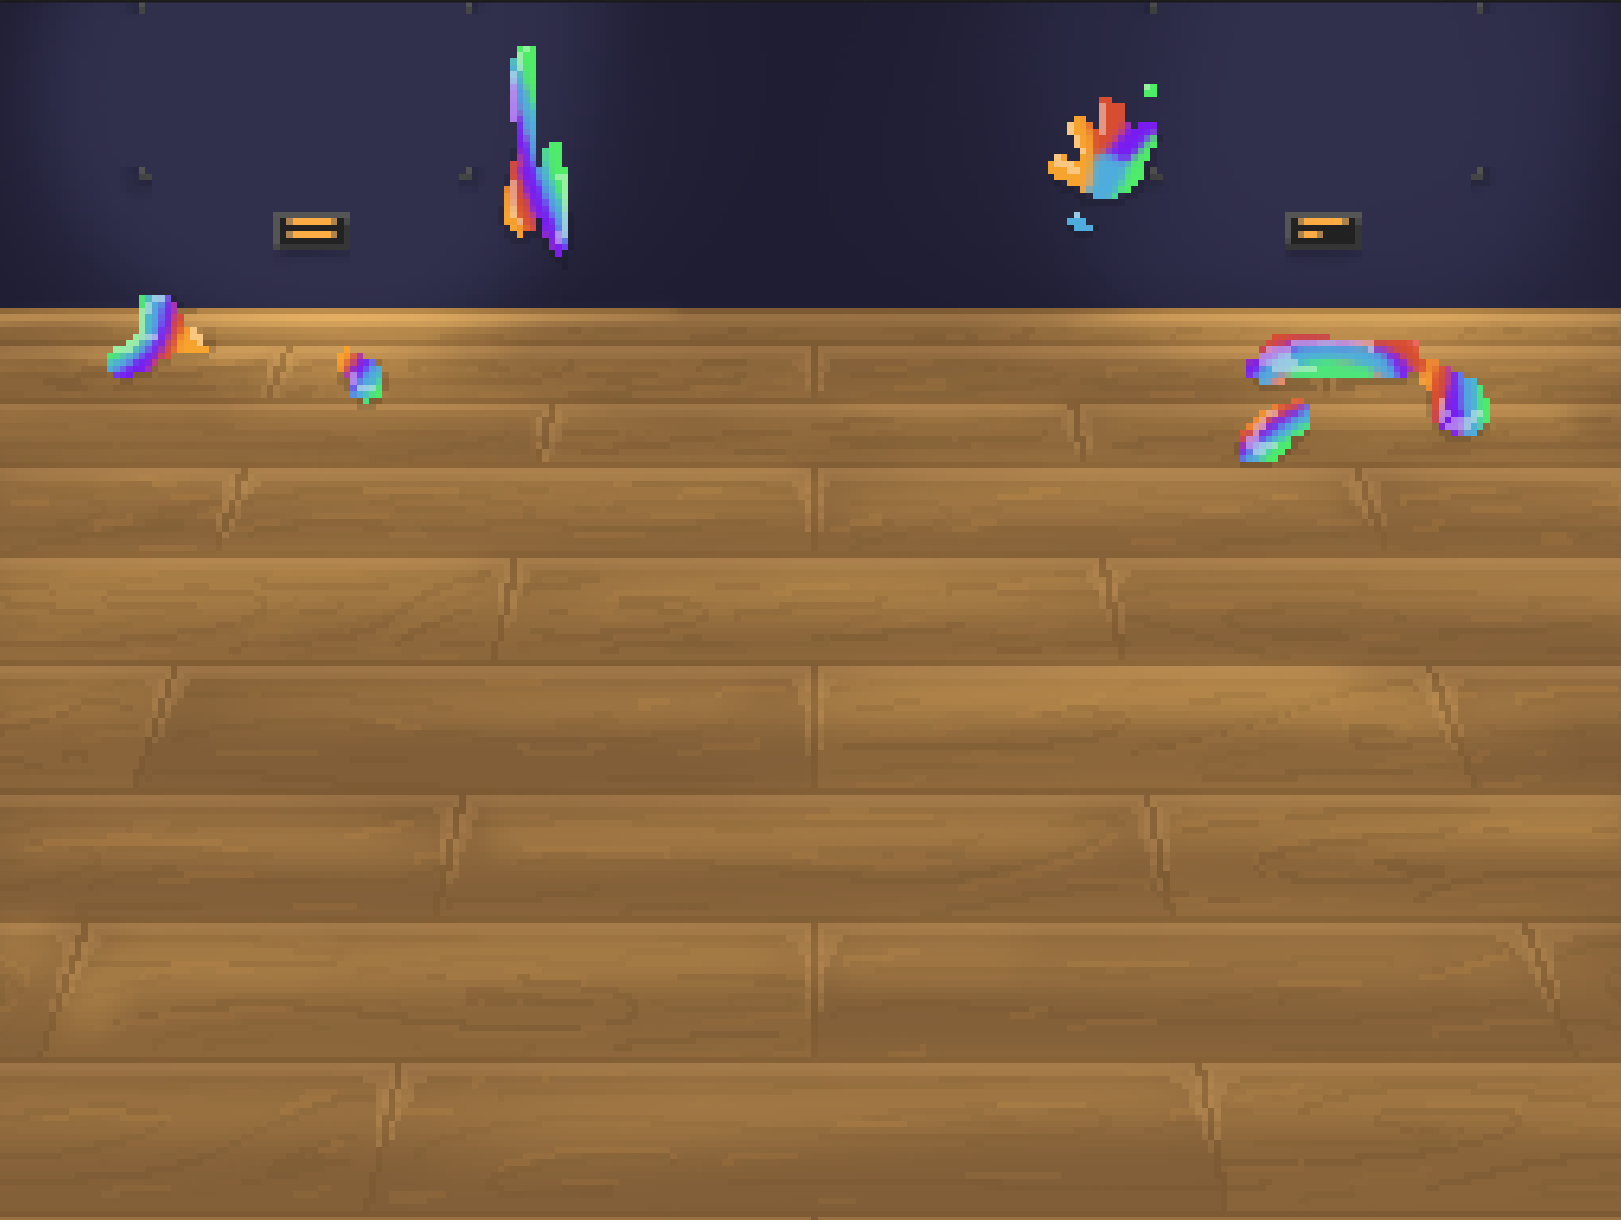
\includegraphics[width=0.5\textwidth]{archivos/bg.png}
  \caption{Fondo de la pantalla de juego que representa la sala de un museo vacía y destrozada.}
  \label{fig:bg_museum}
\end{figure}

\vspace{0.5cm}

Tanto la protagonista como los enemigos tendrán características desproporcionadas tales como gran cabeza, ojos y extremidades, típicas de la estética cartoon. Además, al tratarse de una historia de fantasía y magia, los sprites del juego poseerán \textbf{gran variedad de colores} y bastante saturados, para destacar sobre el fondo y llamar la atención del jugador.



\begin{figure}[htbp]
\centering
  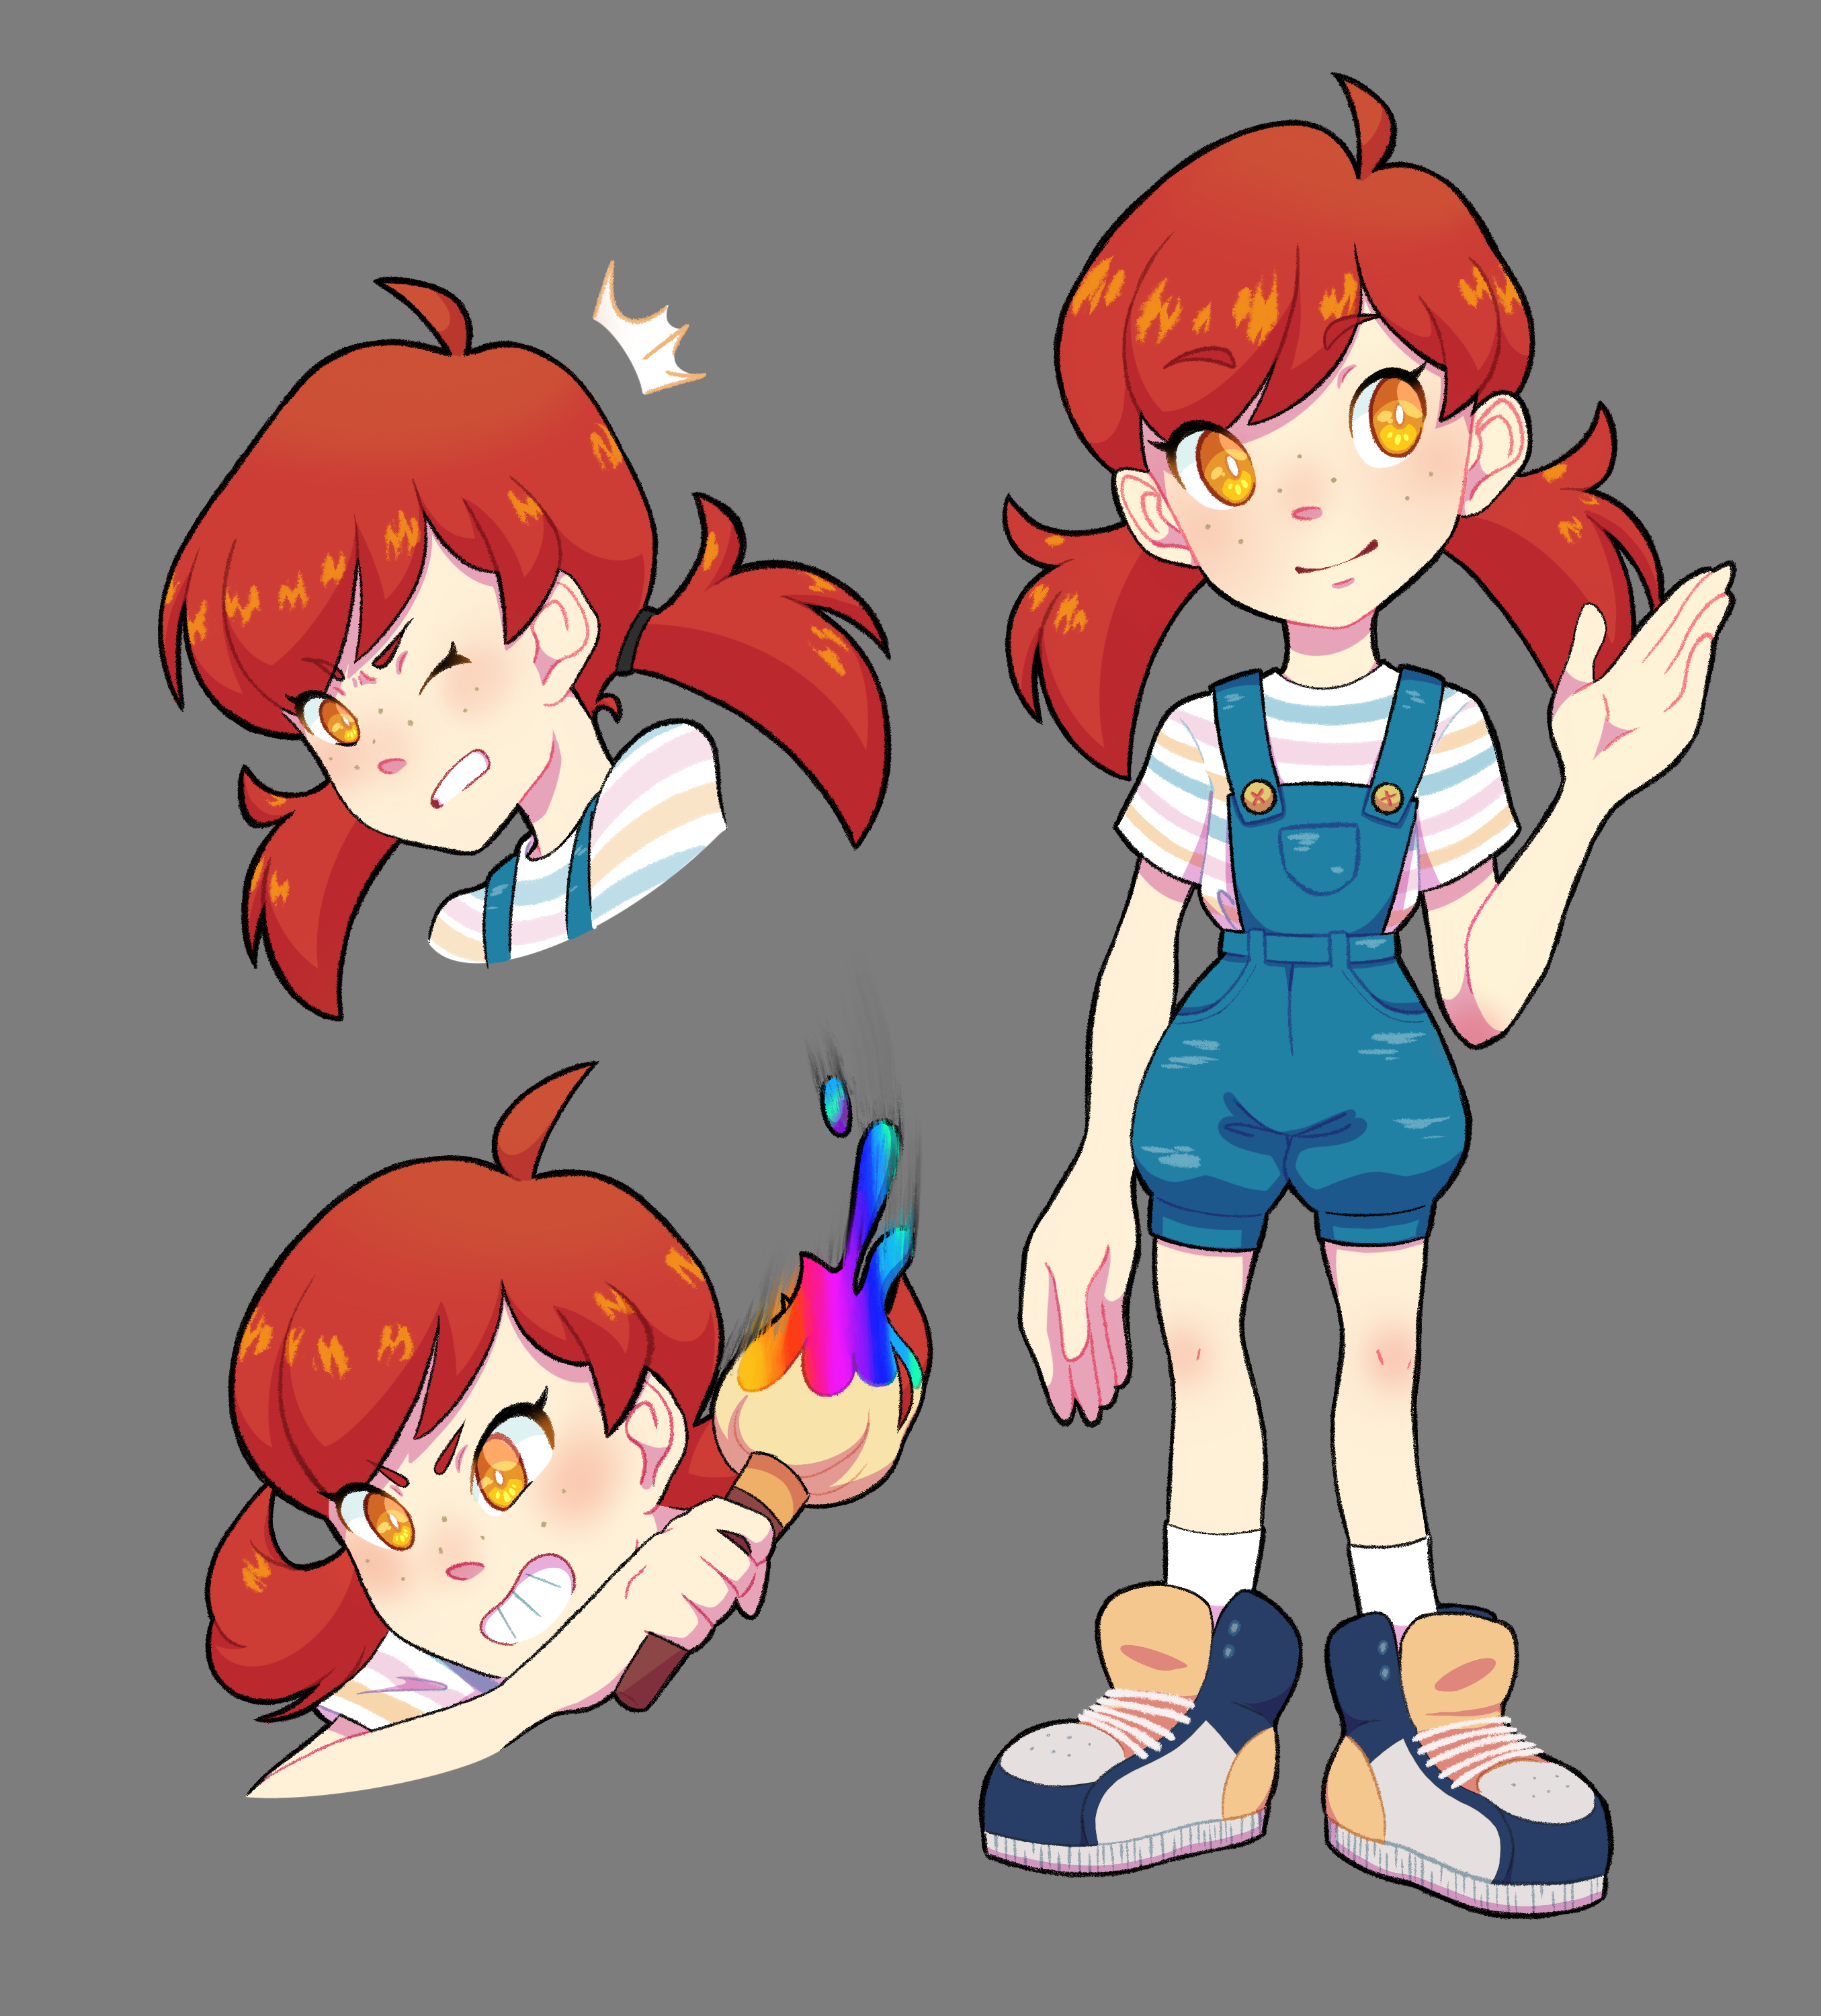
\includegraphics[width=0.45\textwidth]{archivos/cherry.png}
  \caption{Concept art de Cherry, la protagonista del juego, los cuadros.}
  \label{fig:cherry}
\end{figure}

\vspace{0.5cm}

Un toque que posee la ambientación Touch \& Brush y que ayuda a \textbf{unificar el estilo visual} de todo el producto es el uso de \textbf{manchas de pintura de color arcoiris} tratando de simular una pintura mágica. El uso de este recurso se utiliza en diversas ocasiones como por ejemplo, en el pincel Celio, en el logo del juego, en el texto de la pantalla del título y en la mecánica de dibujar en la pantalla táctil y en el propio fondo del museo. Por último, a pesar de que para los gráficos no usaremos una paleta de colores específica, sino más bien todos los que nos permita el hardware, lo que sí haremos será usar el mismo tono lila para hacer las sombras de sprites y fondos. Esto ayudará a cohesionar todos los gráficos y dotar al juego de una consistencia visual.

\vspace{0.5cm}

\begin{figure}[htbp]
\centering
  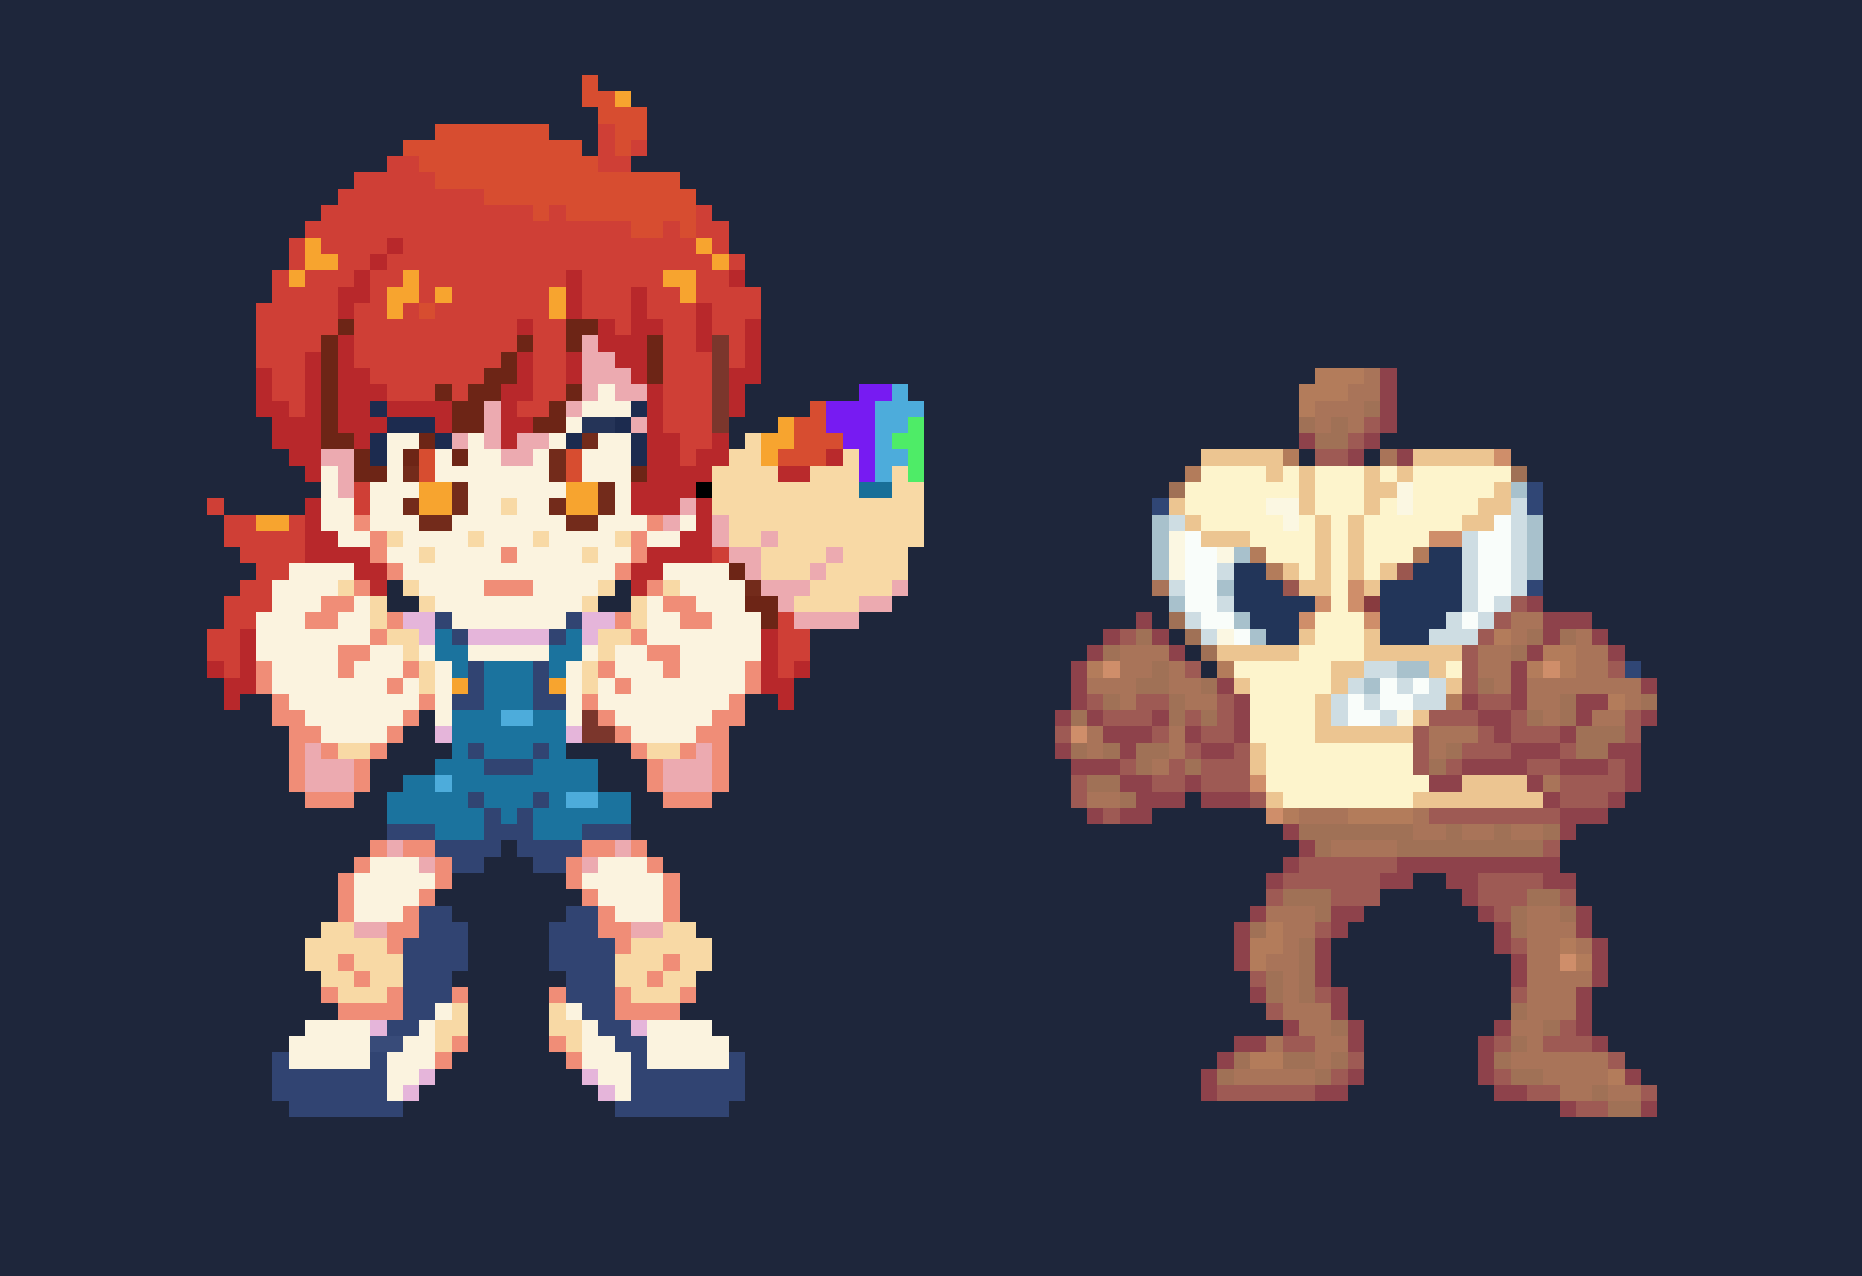
\includegraphics[width=0.5\textwidth]{archivos/sprites.png}
  \caption{Sprites de Cherry y los principales enemigos.}
  \label{fig:sprites_gdd}
\end{figure}

\vspace{1cm}


\subsection{Jugabilidad y mecánicas}

Para \textbf{progresar} en los niveles de Touch \& Brush, el jugador deberá ir \textbf{dibujando el patrón} o conjunto de patrones que los \textbf{enemigos} poseen encima de ellos antes de que éstos lleguen hasta él. El jugador se encontrará en el \textbf{centro superior de la pantalla} y los enemigos aparecerán por los bordes y, al \textbf{alcanzarle}, le \textbf{quitarán una vida}. Este mismo poseerá \textbf{6 vidas} que podrá consultar en todo momento ya que se visualizarán en un \textbf{contador de vidas} en la parte superior izquierda de la pantalla.

\vspace{0.5cm}

Como \textbf{algunos enemigos se moverán más lento que otros}, el reto del jugador es poder \textbf{decidir rápidamente qué patrones dibujar y en qué orden} para avanzar al siguiente nivel con el mayor número de vidas posibles. Además, si somos capaces de \textbf{concatenar varios patrones correctos seguidos} aumentará nuestra \textbf{puntuación}, también visible en cualquier momento en la parte superior derecha de la pantalla.

\vspace{0.5cm}

Por otro lado, si nos encontramos en un nivel de una dificultad superior y hemos perdido más de la mitad de nuestra vida, aparecerá un \textbf{aliado} con un \textbf{patrón de corazón}. Si lo dibujamos correctamente nos aumentará la vida en una unidad.

\vspace{0.5cm}

Al llegar al último nivel encontraremos al \textbf{jefe final}, que debemos derrotar de manera similar a los enemigos normales pero con una serie de fases. Su comportamiento se explicará detalladamente en el apartado de Enemigos.

\vspace{1cm}

\subsection{NPCs}

Dentro del juego distinguiremos tres tipos de NPCs, siendo dos de estos enemigos y uno de ellos un aliado. A continuación se detalla cada uno en profundidad.

\subsubsection{Enemigos comunes}

Como hemos comentado, los enemigos comunes del juego se tratan de los cuadros del museo, que al haberles sido arrebatada su pintura han cobrado vida y se han vuelto furiosos.

\vspace{0.5cm}

Este es el único tipo de enemigo que habrá en los niveles normales del juego y su comportamiento siempre será el mismo: \textbf{ir hacia el jugador} y al alcanzarle le quitará vida. Sin embargo, entre varios enemigos existirán diferencias como por ejemplo la \textbf{velocidad} a la que se mueven, el \textbf{tipo de patrón} que debe dibujar el jugador para matarlos y la\textbf{ posición} desde la que aparecen. Estas características se comentarán más adelante en el apartado de niveles.

\vspace{0.5cm}

Los enemigos podrán aparecer con un patrón de entre \textbf{tres} posibles, los cuales se muestran en la siguiente figura. Se tratan de una l\textbf{ínea horizontal, una línea vertical y un triángulo}. Estos patrones además están representados con \textbf{distintos colores} cada uno para que al usuario, a la hora de visualizarlos en el juego, le sea más fácil distinguirlos.

\vspace{0.5cm}

\begin{figure}[htbp]
\centering
  
\includegraphics[width=0.5\textwidth]{archivos/patterns.png}
  \caption{Tipos de patrones con los que pueden aparecer los enemigos.}
  \label{fig:patterns_enemies}
\end{figure}

\vspace{0.5cm}

\subsubsection{Aliado}

Este NPC tiene la misma apariencia que un enemigo normal, pues también se trata de un cuadro del museo. Sin embargo, \textbf{no es agresivo}, de hecho es beneficioso para el jugador. Su patrón será un dibujo con forma de corazón y si el usuario consigue dibujarlo cuando este aparezca en un nivel, \textbf{aumentará su vida} en una unidad.

\vspace{0.5cm}

Ahora bien, tanto su aparición como su comportamiento no serán igual que los enemigos normales. Este aliado solo aparecerá \textbf{una vez por nivel}, siempre a partir del nivel 3 y siempre que nuestra vida sea igual o inferior a la mitad. Además, no correrá hacia el jugador, sino que aparecerá desde el borde izquierdo de la pantalla y \textbf{avanzará en línea recta hasta la mitad de la pantalla}, donde se detendrá.

\vspace{0.5cm}

\begin{figure}[htbp]
\centering
  
\includegraphics[width=0.3\textwidth]{archivos/heart.png}
  \caption{Tipos de patrones con los que pueden aparecer los enemigos.}
  \label{fig:patterns_heart}
\end{figure}

\vspace{0.5cm}

\subsubsection{Jefe}

Este enemigo se trata del jefe final del juego, el cual representa al \textbf{cuadro más prestigioso} y valorado del museo. En cuanto a su apariencia, es igual que los enemigos normales pero de mayor tamaño, ojos rojizos y porta una corona de rey.

\vspace{0.5cm}

Se podrá encontrar después de haber superado el último nivel y su comportamiento será distinto. En primer lugar, se encontrará en la parte derecha de la pantalla, avanzando hacia la izquierda donde se encuentra el jugador. También, su daño será mayor, quitando de un solo golpe 2 corazones. 

\vspace{0.5cm}

La forma en la que debemos matarlo también será diferente a los demás enemigos. Su comportamiento estará dividido en \textbf{3 fases}, y en cada una de ellas generará una \textbf{secuencia de 5 patrones} que el jugador deberá dibujar \textbf{en orden} mientras dicho jefe se va moviendo a una velocidad concreta hacia este. Si el jugador lo logra, el jefe volverá a su posición inicial, pasando a la siguiente fase, donde aumentará su velocidad y la secuencia de patrones volverá a generarse.

\vspace{0.5cm}

\begin{figure}[htbp]
\centering
  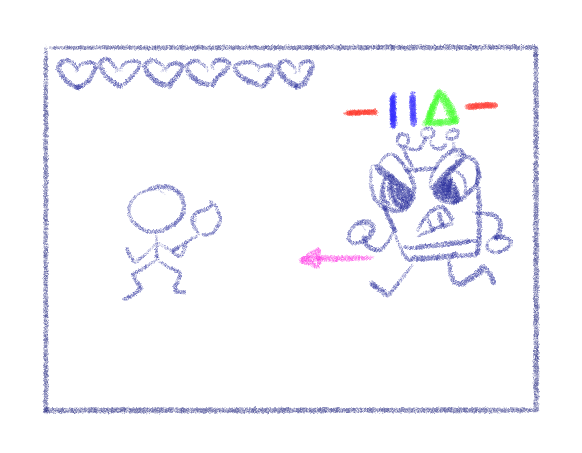
\includegraphics[width=0.5\textwidth]{archivos/mockup_boss.png}
  \caption{Mockup del enfrentamiento con el jefe.}
  \label{fig:mockup_boss}
\end{figure}

\vspace{1cm}

\subsection{Niveles}

El juego constará de \textbf{4 niveles normales} y \textbf{un nivel de jefe final}.

\vspace{0.5cm}

En cuanto a los niveles normales, visualmente no serán muy distintos entre sí, pero sí que hay \textbf{5 parámetros} que podemos ajustar para dotar a los niveles de Touch \& Brush de una curva de complejidad y aprendizaje interesantes.

\vspace{0.5cm}

En primer lugar, tenemos el \textbf{tiempo} que transcurre entre la aparición de enemigos. A medida que avancemos en los niveles, este tiempo se irá reduciendo para que aparezcan enemigos con más frecuencia y el jugador deba dibujar los patrones más rápido.

\vspace{0.5cm}

Después, tenemos la \textbf{posición} desde la que aparecen los enemigos y la \textbf{velocidad} a la que se mueven. Al encontrarse el jugador en el centro de la pantalla, los enemigos podrán salir desde 6 posiciones distintas y dirigirse hacia él. Estas posiciones son: esquinas superiores derecha e izquierda, centro derecha e izquierda y esquinas inferiores derecha e izquierda. En cuanto a la velocidad, es interesante que algunos enemigos sean capaces de moverse más rápido que otros para despistar al jugador. Por ejemplo, si sale un enemigo desde un lado a una velocidad lenta el jugador se fijará en ese e intentará derrotarlo, pero entonces es cuando aparece un enemigo que se mueve más rápido, le alcanza antes de que pueda darse cuenta o reaccionar y le quita una vida.

\clearpage

\begin{figure}[htbp]
\centering
  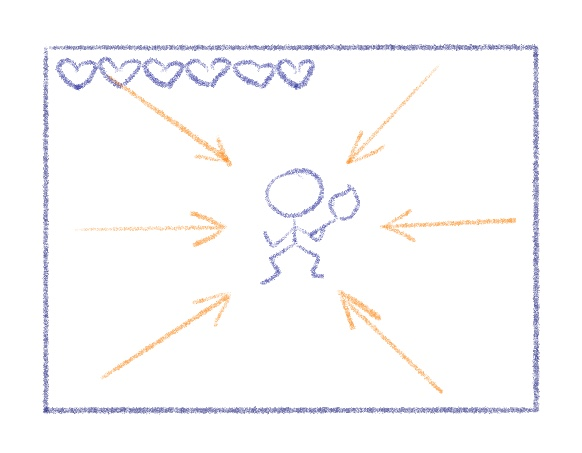
\includegraphics[width=0.4\textwidth]{archivos/pos_enemies.jpg}
  \caption{Posiciones iniciales desde las que pueden aparecer enemigos.}
  \label{fig:pos_enemies}
\end{figure}

Por otro lado tenemos el \textbf{número de enemigos que debemos derrotar} para pasar al siguiente nivel, que irá aumentando según avancemos. Y por último, tenemos la \textbf{complejidad de los patrones} de los enemigos. Es bastante más fácil de dibujar una línea recta que un triángulo, así que los primeros niveles comenzarán con esos patrones más simples y a medida que avancemos se incorporarán los más complejos.

\vspace{0.5cm}

Así pues, una vez explicado esto, los 4 niveles de Touch \& Brush tendrían las siguientes características:

\begin{itemize}
  \item \textbf{Nivel 1:} Enemigos lentos que únicamente aparecen por los laterales centrales de la pantalla, moviendose lento y sus patrones serán la línea horizontal y vertical. Será necesario derrotar aun total de 6 enemigos para pasar al siguiente nivel y la frecuencia con la que estos aparecen será la más baja.
  
    \item \textbf{Nivel 2:} En este nivel se incorporan los enemigos que salen desde las esquinas superiores e inferiores, llevando estos una velocidad mayor. Además, el número de enemigos a derrotar aumenta a 10 así como aumenta también la frecuencia con la que éstos aparecen.
    
    
    \item \textbf{Nivel 3:} Se mantienen las mismas posiciones y velocidades de los enemigos, así como sus patrones. Aumenta el número de enemigos que derrotar a 13 y también lo hace la frecuencia con la que éstos aparecen. Se incorpora el aliado que te permite recuperar vida.
    
    
    \item \textbf{Nivel 4:} Nuevamente, aumenta el número de enemigs que derrotar a 16 y la frecuencia con la que aparecen. Además también aparecen los enemigos con patrón de triángulo.
    
\end{itemize}

\subsection{Controles}

En cuanto a los controles, al tratarse de un juego para una consola con pantalla táctil la gran mayoría de interacciones tanto para el \textbf{gameplay principal} como la \textbf{selección de opciones en los menús} se harán mediante esta. No obstante, cabe destacar que para \textbf{abrir el menú de pausa} se pulsará el botón \textbf{START}.

\subsection{Estados del juego}
 Aquí veremos un resumen de todos los estados del juego, así como el flujo entre ellos para que a la hora de desarrollar tengamos en cuenta desde qué estados se puede llegar a uno en concreto. 
 
 \vspace{0.5cm}
 
 En la siguiente imágen se puede observar dicho resumen, y más adelante veremos las pantallas que se corresponden con cada estado.
 
  \vspace{0.5cm}
 
 \begin{figure}[htbp]
\centering
  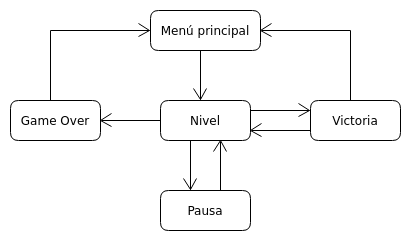
\includegraphics[width=0.5\textwidth]{archivos/diagramaflujo.png}
  \caption{Diagrama de flujo entre estados}
  \label{fig:diagflujo}
\end{figure}

 \vspace{0.5cm}

Al inciar el juego se cargará el \textbf{menú principal}, que nos dará la opción de empezar a jugar desde el primer nivel ya que no habrá guardado de partida. Si completamos un nivel, pasaremos al estado de \textbf{victoria}, que nos mostrará un mensaje de que hemos completado el nivel y nos dará la opción tanto de volver a jugar ese nivel, continuar al siguiente o volver al menú principal.

 \vspace{0.5cm}

Por otro lado, si mientras jugamos perdemos, independientemente del nivel en el que nos encontrasemos pasaremos al estado de \textbf{fin de partida}, que nos mostrará un mensaje de que hemos muerto, la puntuación obtenida y únicamente nos permitirá volver al menú principal.

 \vspace{0.5cm}

Por último, mientras estemos jugando a cualquier nivel podremos cambiar al \textbf{estado de pausa} si deseamos dejar en espera nuestro juego y así mismo desde este menú de pausa podremos volver al estado donde dejamos la partida.

 \vspace{0.5cm}

\subsection{Pantallas}

A continuación se muestran una serie de \textbf{bocetos de pantallas} asociadas a los distintos estados del juego, así como también los elementos visuales que estos poseen, qué información nos dan y si son interactuables.

 \vspace{0.5cm}
 
 En primer lugar, la pantalla del menú principal. En ella no habrán muchos elementos, teniendo en la pantalla superior el logo del juego y, en la inferior un mensaje que nos indicará que debemos tocar la pantalla para comenzar a jugar. Además, en esta misma pantalla también se mostrará el nombre del autor del juego.
 
  \begin{figure}[htbp]
\centering
  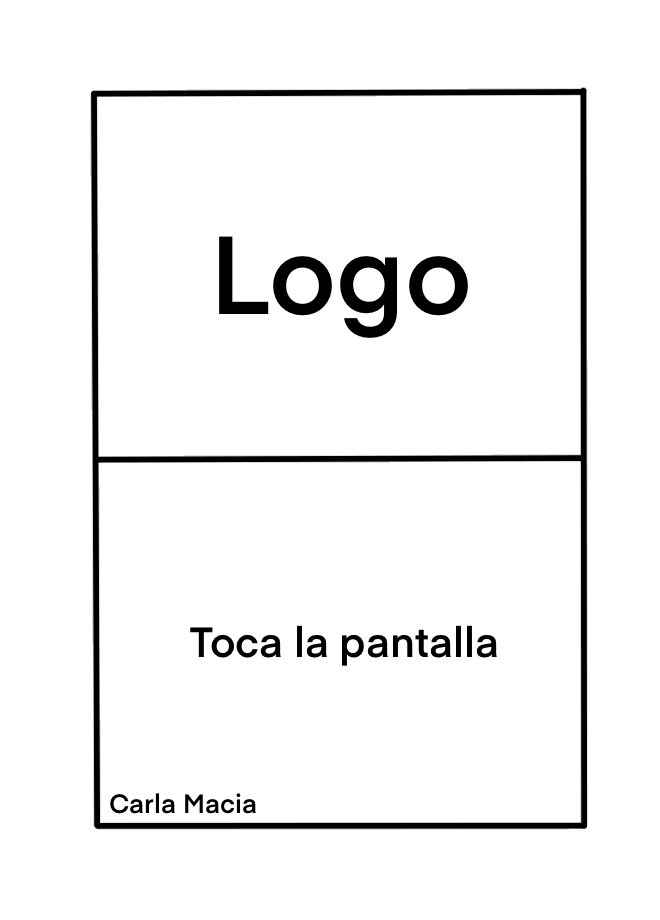
\includegraphics[width=0.3\textwidth]{archivos/mockup_title.png}
  \caption{Mockup de la pantalla de título}
  \label{fig:mockup_title}
\end{figure}

 \vspace{0.5cm}
 
 Por otro lado tenemos la pantalla de nivel, siendo esta donde el jugador más tiempo pasará y más información le aportará. En la pantalla superior, haciendo uso de sprites se podrán visualizar los enemigos moviendose por la pantalla, el jugador y la vida de éste mismo. Además, en la parte derecha superior tendremos un contador que nos indicará nuestra puntuación y se irá actualizando mientras jugamos.
 
 \vspace{0.5cm}
 
 En la pantalla inferior es donde el jugador irá dibujando los patrones, por ello mediante un fondo simularemos una especie de lienzo y cuando el jugador esté tocando la pantalla táctil iremos dibujando el trazo que éste realiza.
 
 \clearpage
 
   \begin{figure}[htbp]
\centering
  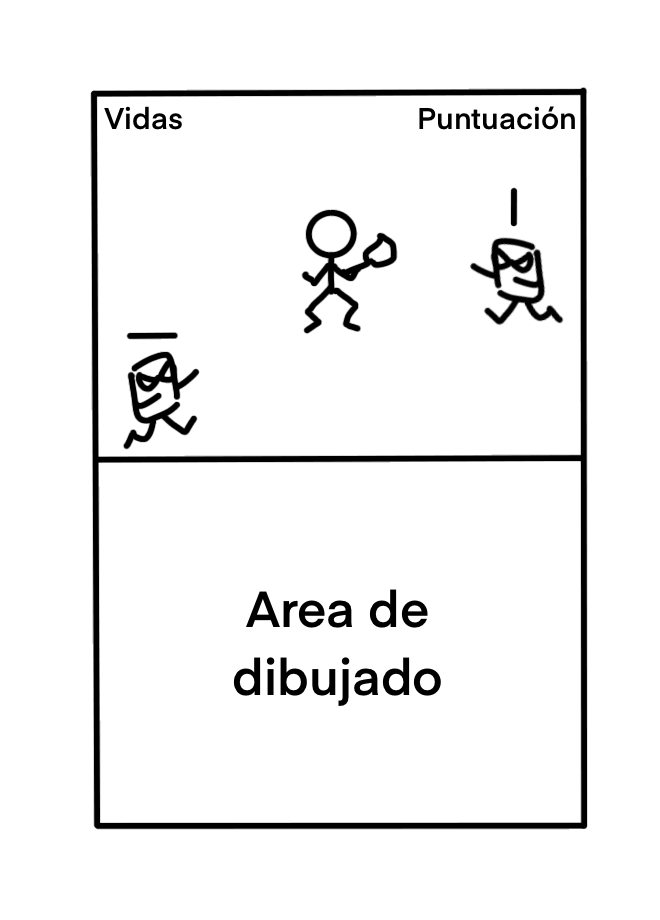
\includegraphics[width=0.3\textwidth]{archivos/mockup_game.png}
  \caption{Mockup del juego}
  \label{fig:mockup_game}
\end{figure}
 
Después, en cuanto al los estados de victoria o final de partida, ambos son muy similares. En la pantalla superior ambos mostrarán un mensaje indicando si han ganado o perdido, y después un texto con la puntuación obtenida. En la pantalla inferior, habrá un botón común en ambos para volver al menú principal y otro en el caso de la pantalla de victoria que nos llevará al siguiente nivel. Estos botones serán interactuables tocando sobre ellos en la pantalla táctil. Cabe destacar también, que en caso de habernos pasado el juego entero el botón de pasar al siguiente nivel no estará disponible.

\clearpage
 
    \begin{figure}[htbp]
\centering
  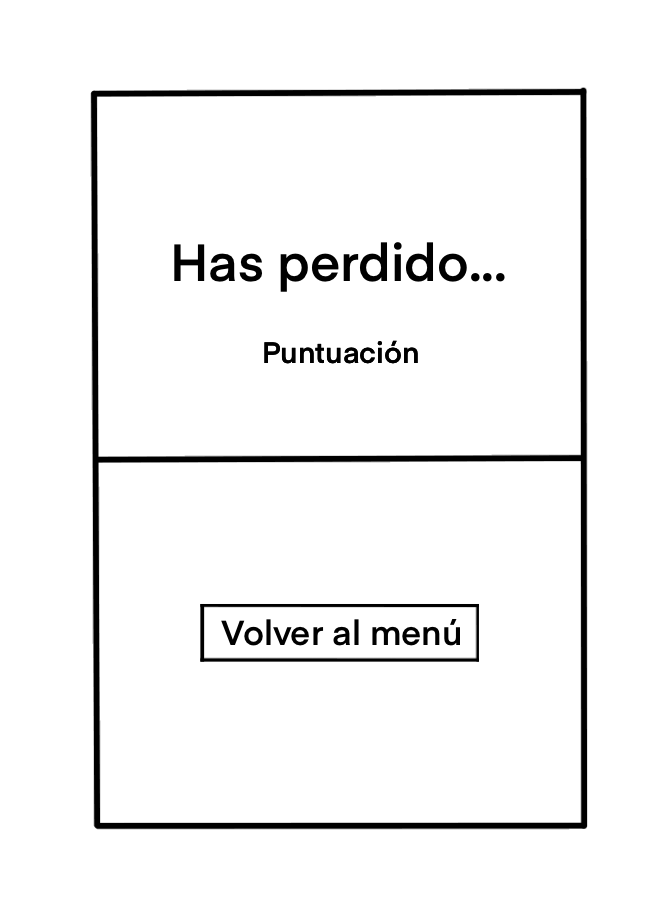
\includegraphics[width=0.3\textwidth]{archivos/mockup_gameover.png}
  \caption{Mockup de la pantalla de fin de partida}
  \label{fig:mockup_gameover}
\end{figure}

   \begin{figure}[htbp]
\centering
  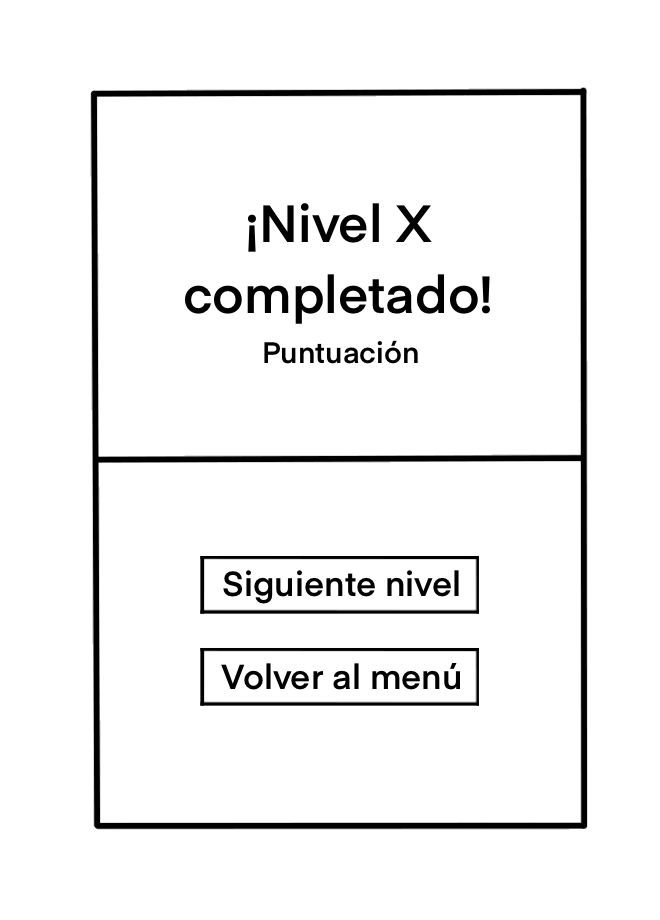
\includegraphics[width=0.3\textwidth]{archivos/mockup_win.png}
  \caption{Mockup de la pantalla de victoria}
  \label{fig:mockup_win}
\end{figure}

Por último, la pantalla de pausa como ya hemos comentado no aportará gran información al usuario. Esta simplemente le mostrará en la pantalla superior un texto de que ha pausado la partida y en la pantalla inferior un botón para reanudarla.

  \begin{figure}[htbp]
\centering
  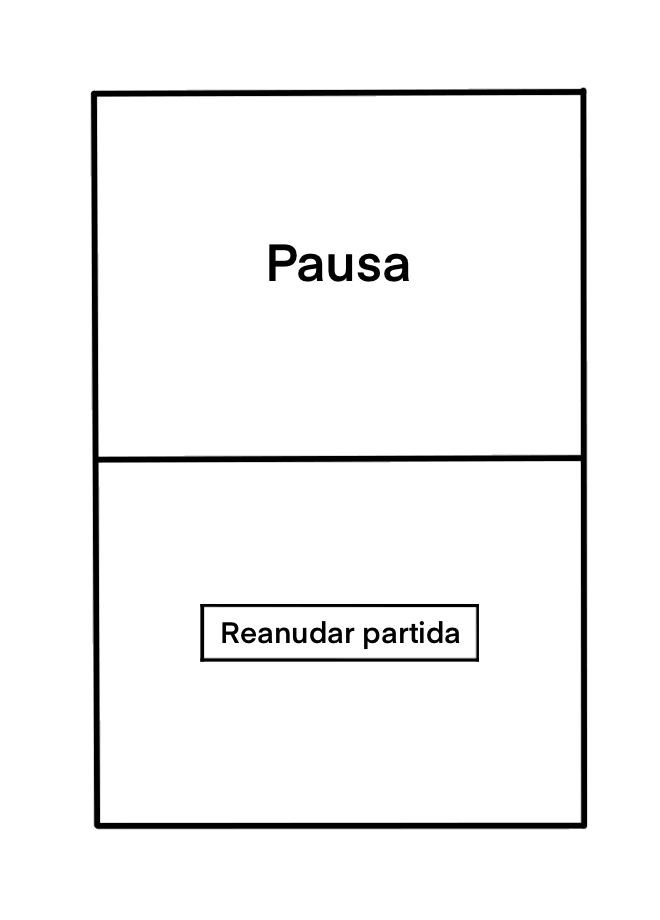
\includegraphics[width=0.3\textwidth]{archivos/mockup_pause.png}
  \caption{Mockup de la pantalla de pausa}
  \label{fig:mockup_pause}
\end{figure}

\begin{comment}
\subsection{Mínimo producto viable}

Todo este diseño está pensado para que, en el mejor de los casos se puedan implementar todas las mecánicas, tipos de enemigos, pantallas, etc. en el tiempo disponible de desarrollo pero tristemente es poco probable que así sea.

\vspace{0.5cm}

Surgirán problemas, tanto externos como internos, de eso no cabe duda, y no queremos vernos en la situación de estar a pocas semanas de la fecha final y \textbf{solo tener un prototipo}. Es por ello que hay que estar preparado para eso y definir una versión simplificada, que siga funcionando como juego y sea un \textbf{producto cerrado} de principio a fin, algo que la gente pueda probar para ver si le gustan las mecánicas o no y a partir de ahí \textbf{trabajar iterativamente} sobre ello añadiéndole las funcionalidades explicadas anteriormente con un \textbf{orden de prioridad}.

\vspace{0.5cm}

Así pues, el mínimo producto que se plantea es el siguiente:

\vspace{0.5cm}

Tendrá un \textbf{único y primer nivel}, donde los enemigos que aparezcan solo tengan \textbf{un patrón} que será al azar entre \textbf{dos tipos distintos} (horizontal y vertical).

\vspace{0.5cm}

Se implementará la \textbf{muerte} del jugador, así como la \textbf{victoria}, de modo que el juego pueda \textbf{rejugarse} tantas veces como se quiera. No obstante, no sería necesario implementar aún las respectivas pantallas de fin de juego y victoria, con volver a la pantalla principal bastaría.

\vspace{0.5cm}

Por último carecería de animaciones y sonido, pues implementar las \textbf{mecánicas} es \textbf{prioritario} frente a perfeccionar lo visual. Sin embargo, sí que se implementará el dibujado del \textbf{rastro del lápiz en la pantalla táctil}, así nos servirá como \textbf{método de depurado} en caso de que el reconocimiento de gestos nos de problemas.

\vspace{0.5cm}

En la siguiente imágen se muestra un mockup de lo que sería el mínimo producto viable:

\vspace{0.5cm}

\begin{figure}[htbp]
\centering
  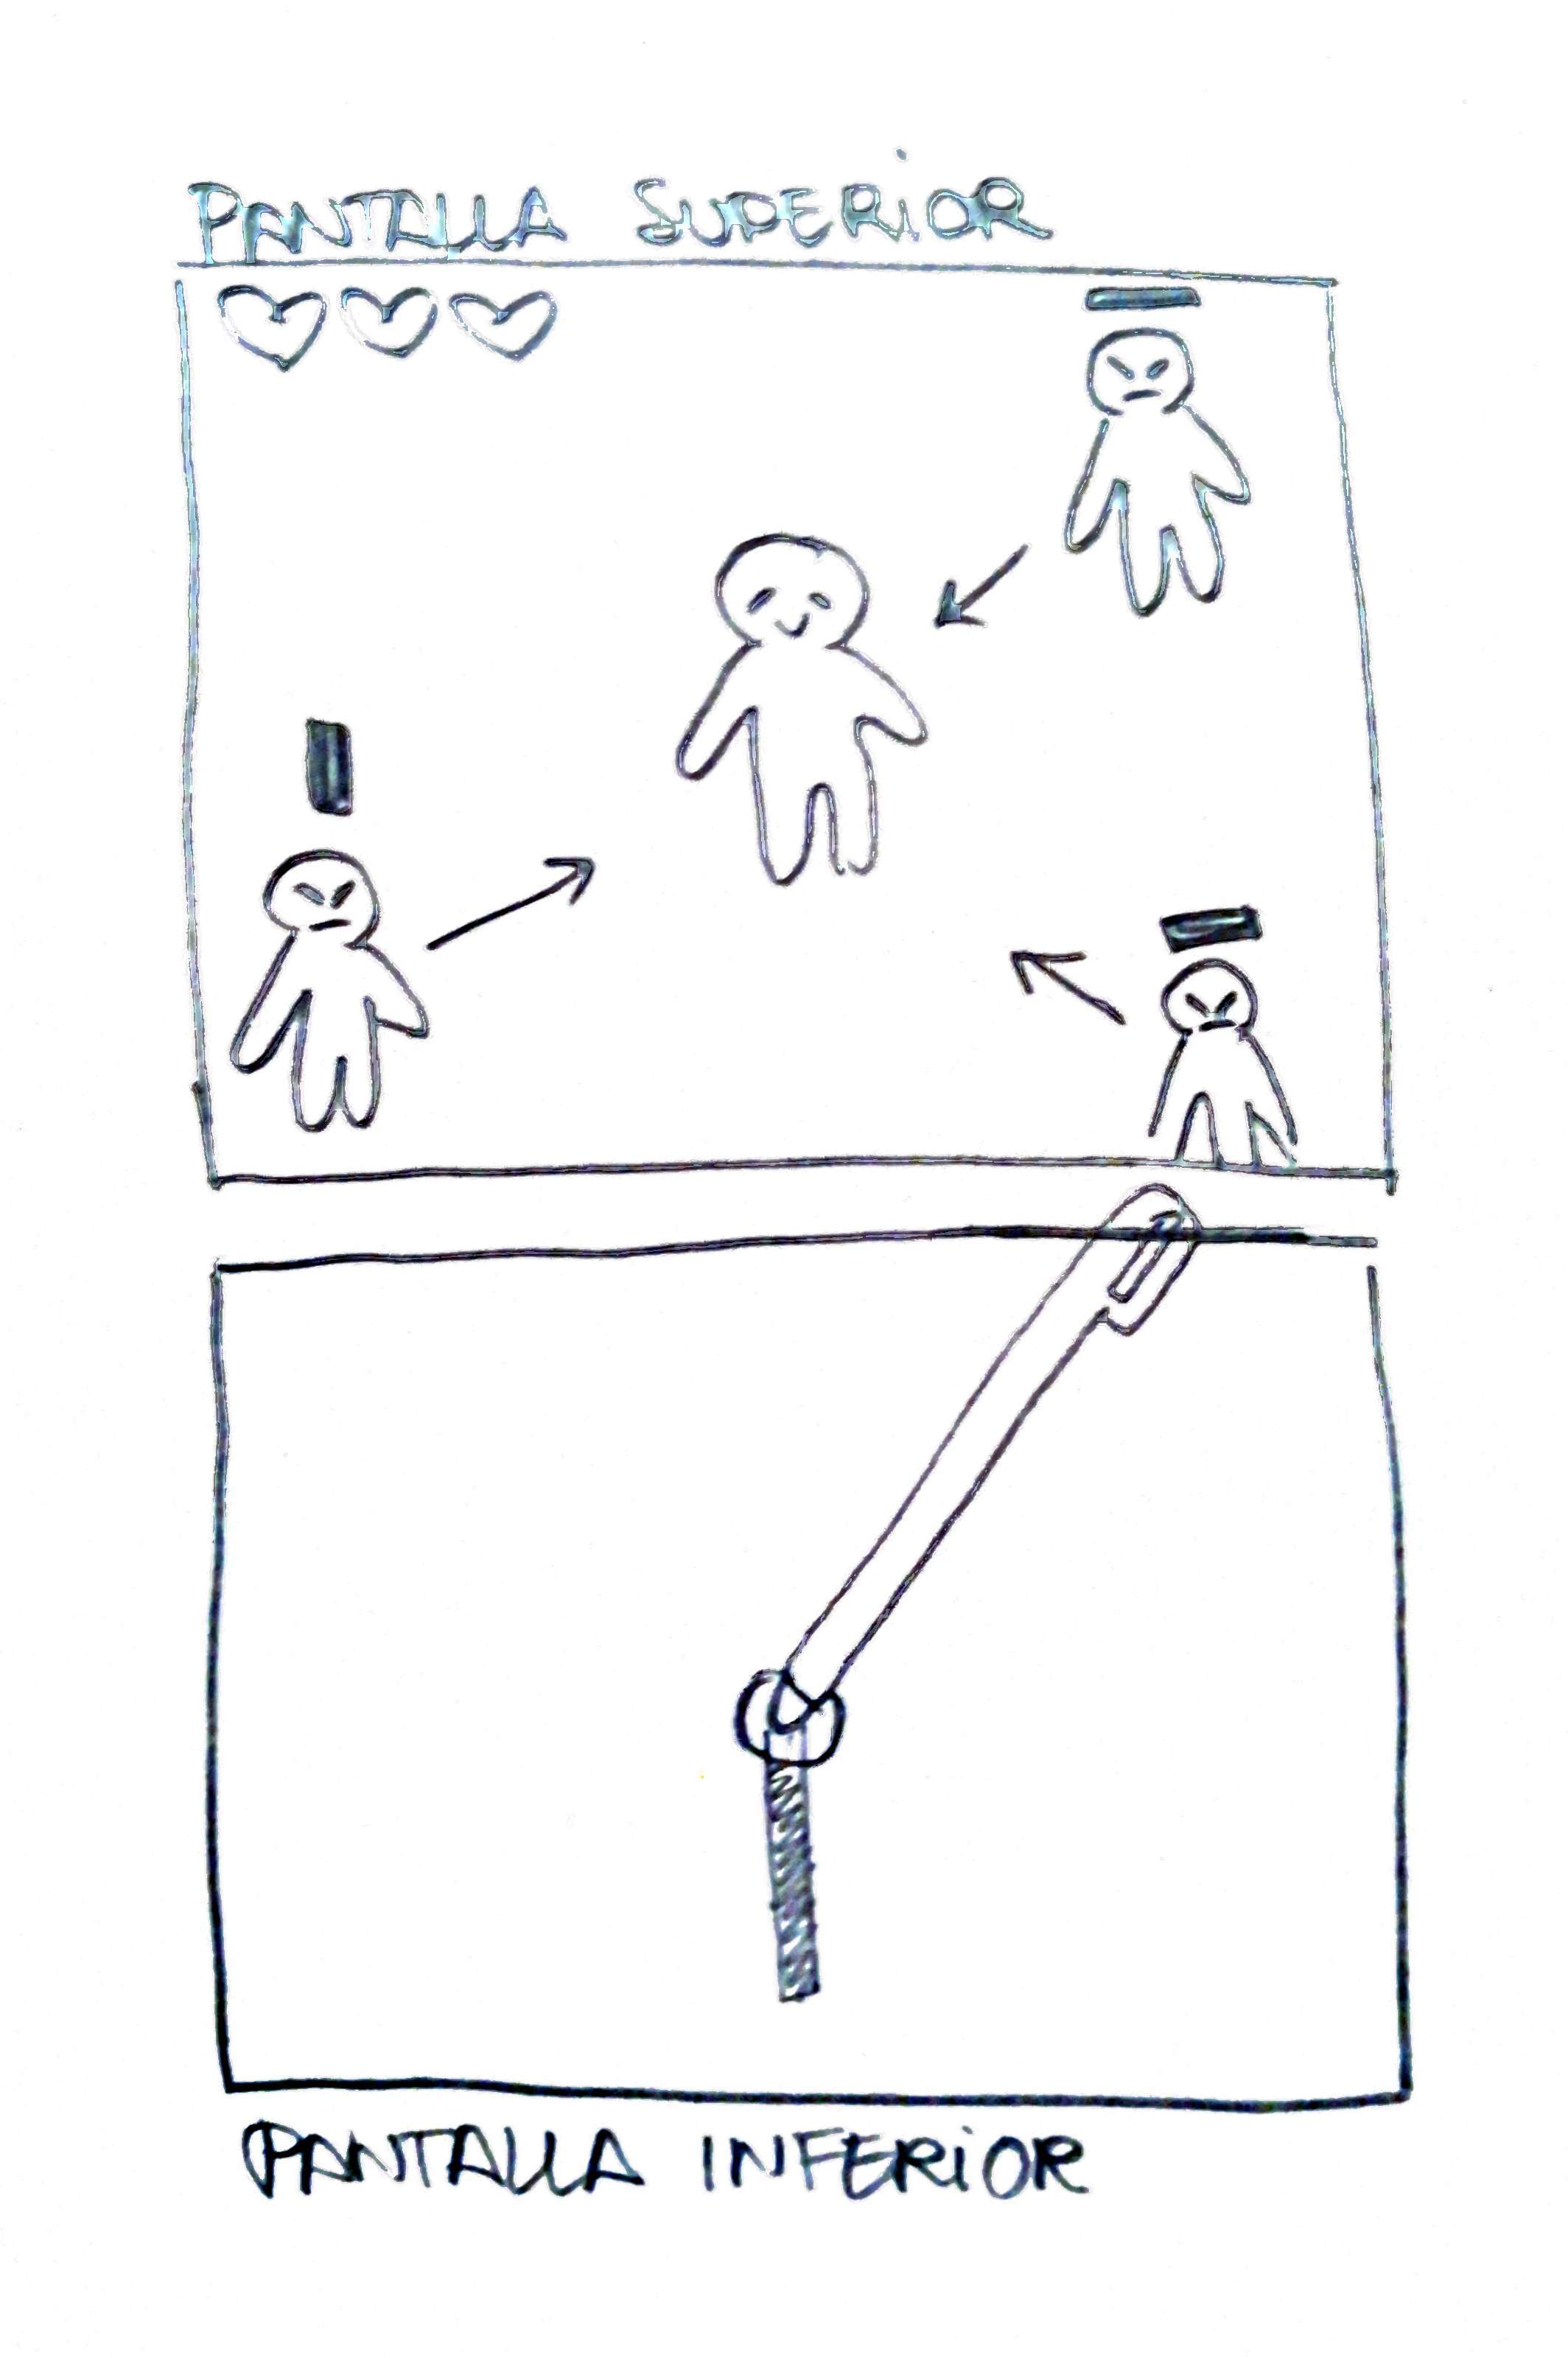
\includegraphics[width=0.4\textwidth]{archivos/minimoprod.jpg}
  \caption{Concepto del mínimo producto viable.}
  \label{fig:minimoprod}
\end{figure}
\end{comment}
